% !TEX root = ../main.tex

% 预习报告	
\setcounter{section}{0}
\section{APL1-1-A 电阻热噪声及玻尔兹曼常量测量 \\ Preview Report}


%---------------------------------------------------------------------
% 实验目的
\subsection{Purpose}
\begin{enumerate}
	\item \textbf{核心目的：通过测量电阻热噪声精密测量玻尔兹曼常量}；
	\item 其它：
	\begin{enumerate}
		\item 通过实验了解热噪声的特征，理解热噪声的本质及其统计特征；
		\item 测出玻尔兹曼常量；
		\item 学习 VISA 接口协议，通过 LabVIEW 设置锁相放大器参数和进行数据采集。
	\end{enumerate}
\end{enumerate}


%---------------------------------------------------------------------
% 仪器用具
\subsection{Instruments \& Equipment}
\begin{table}[h]
	\centering
	\caption{热噪声测（玻尔兹曼常量）量仪器用具}
	\begin{tabular}{ccccc}
		\hline
		\textbf{编号} & \textbf{仪器用具名称} & \textbf{数量} & \textbf{主要参数（型号、规格等）} & \textbf{备注} \\ \hline
		1 & 锁相放大器 & 1 & OE1022 & \\ 
		2 & 示波器 & 1 & RIGOL DS2202A & \\ 
		3 & 数字多用表 & 1 & RIGOL DM3058E、MS6514 & \\ 
		4 & 测温仪 & 1 & MS6514 & \\ 
		5 & PC 机 & 1 & LabVIEW 环境及有 VISA 接口协议 & \\ 
		6 & 可变温样品盒（带 BNC 接头） & 1 & 6.6k$\Omega$、13k$\Omega$、41k$\Omega$、66k$\Omega$、98k$\Omega$、144k$\Omega$ & 任选其一 \\ \hline
	\end{tabular}
\end{table}


%---------------------------------------------------------------------
% 原理概述
\subsection{Principle}
\begin{enumerate}
	\item 约翰逊-奈奎斯特噪声
	
	\textbf{约翰逊-奈奎斯特噪声（Johnson–Nyquist noise，即我们熟知的热噪声）}是由于电导体内的电荷载流子（通常为电子）在平衡状态下的热扰动所产生的电子噪声。
	
	这种现象与施加电压无关。热噪声存在于所有电路中，在某些灵敏的电子设备（如无线电接收器）中，热噪声会淹没弱信号，成为限制电子测量仪器灵敏度的主要因素。热噪声与绝对温度成正比，因此一些灵敏的电子设备（如射电望远镜的接收器）被冷却至低温状态以改善其信噪比。
	
	热噪声的通用统计物理推导称为\textbf{涨落-耗散定理}（详见后），该定理使用广义的电阻抗或广义的电极化率来表征介质的性质。
	
	\begin{figure}[htbp]
		\centering
		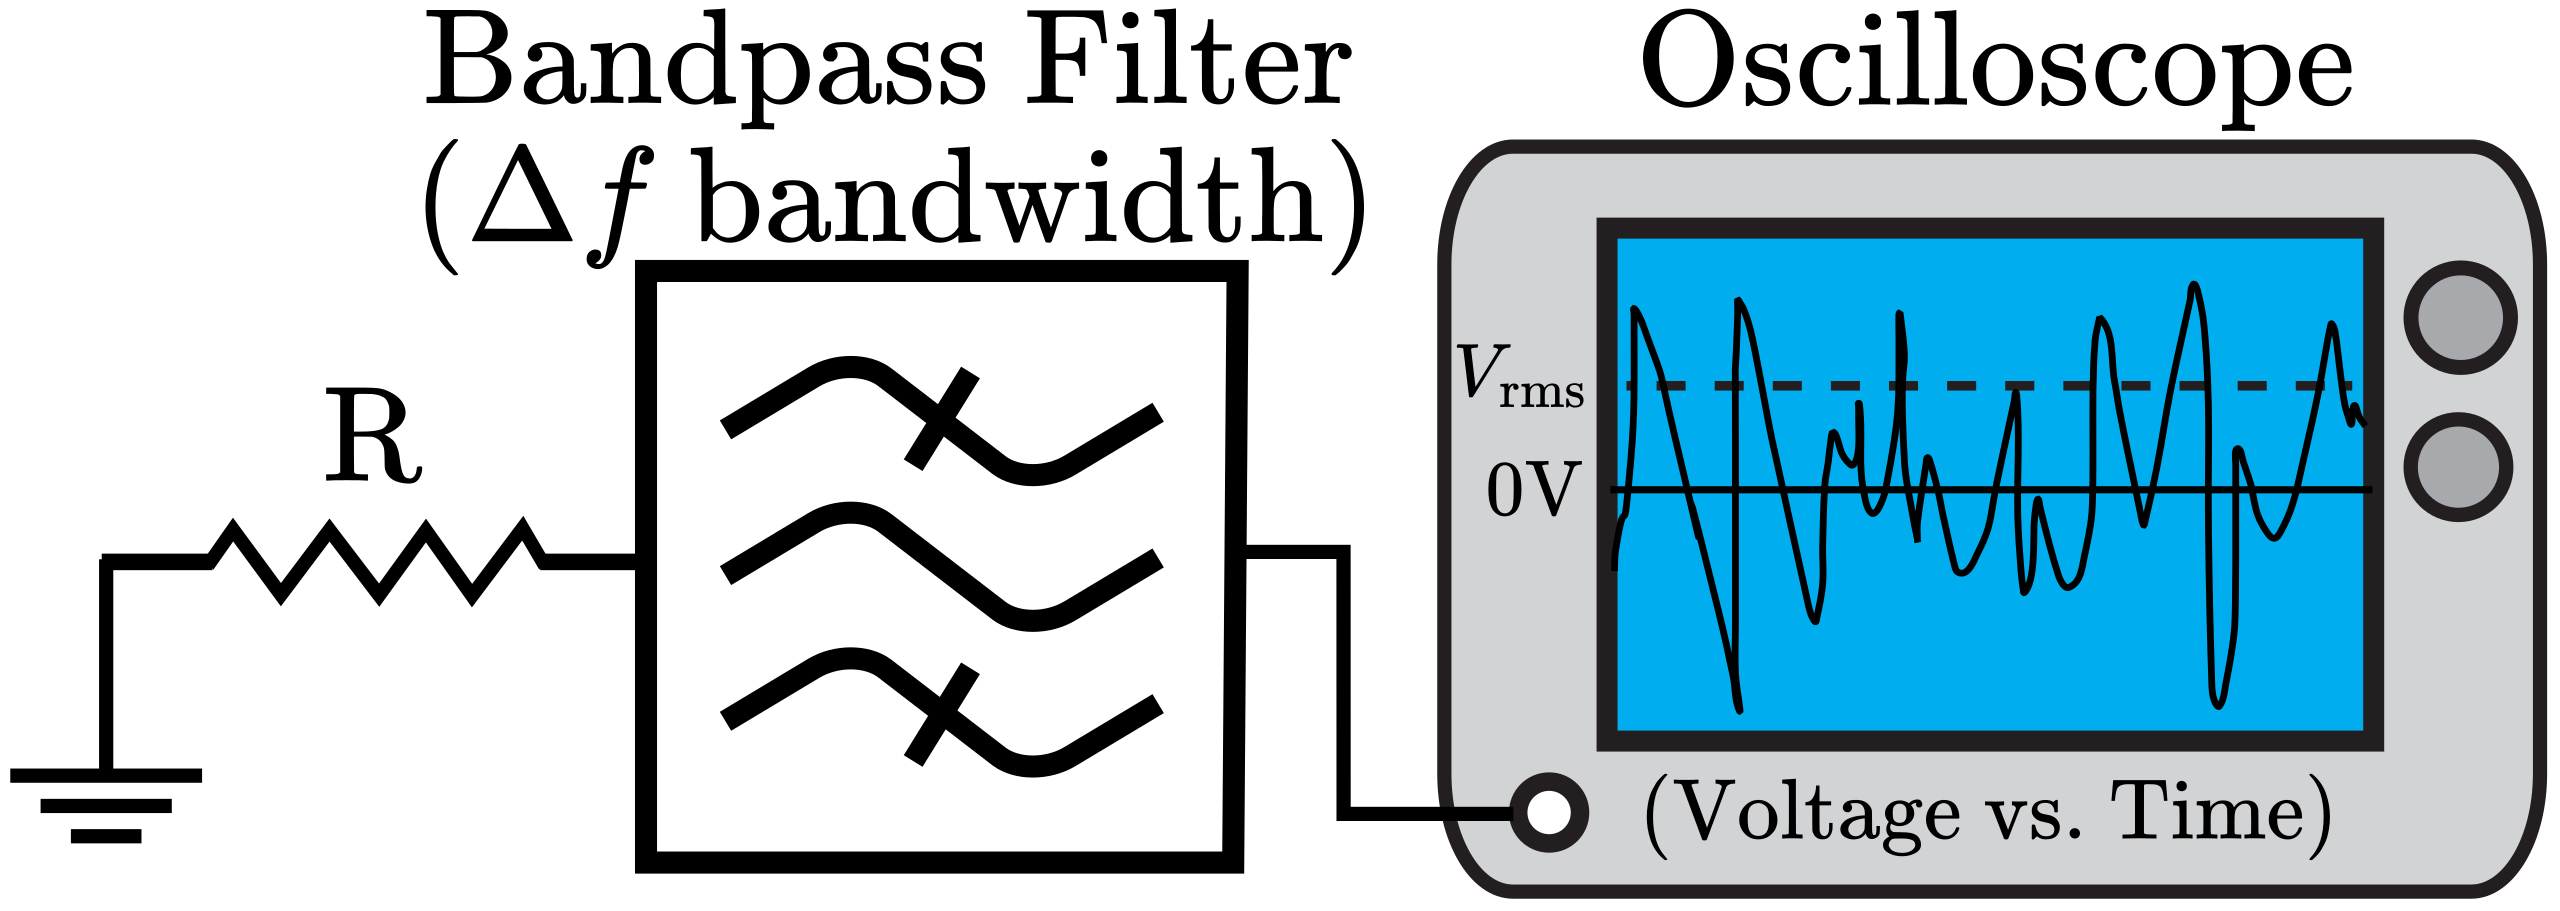
\includegraphics[width=0.5\linewidth]{images/Oscilloscope-setup-johnson-noise}
		\caption{约翰逊于1927年的实验表明，如果温度为$T$的电阻$R$的热噪声被限制在带宽$\Delta f$内，则其均方根电压($V_{\text{rms}}$)一般为$\sqrt{4 k_\text{B} T R \Delta f}$，其中$k_\text{B}$为玻尔兹曼常数。（来自\cite{a}）}
		\label{fig:oscilloscope-setup-johnson-noise}
	\end{figure}
	
	\begin{figure}[htbp]
		\centering
		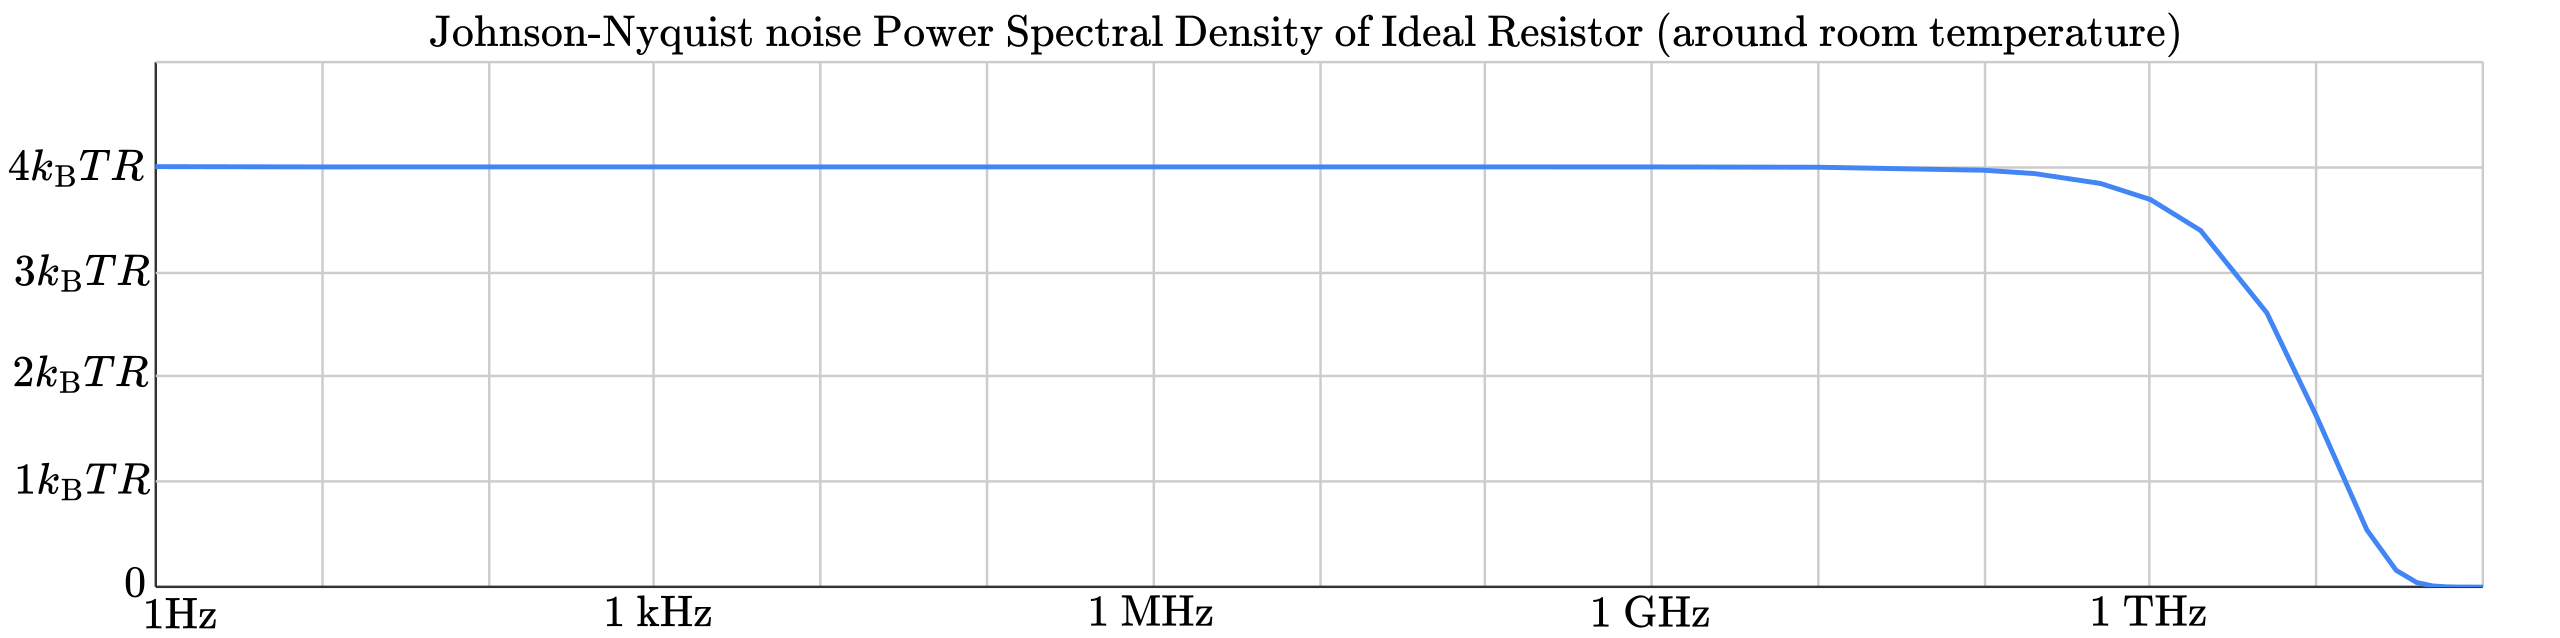
\includegraphics[width=0.75\linewidth]{images/Johnson-nyquist-noise-power-spectral-density-of-ideal-resistor}
		\caption{约翰逊-奈奎斯特噪声的功率谱密度在每单位频率下接近常数，即$4k_\text{B}T R$，但由于量子效应，在高频（室温下为THz）时功率谱密度会衰减至零。该图的横轴使用对数刻度，每条竖线对应频率（以Hz为单位）的10次幂。（来自\cite{a}）}
		\label{fig:johnson-nyquist-noise-power-spectral-density-of-ideal-resistor}
	\end{figure}
	
	\begin{enumerate}
		\item 中等频率的理想电阻噪声
		
		\begin{ubox}{}
			约翰逊的实验发现，带宽为$\Delta f$的频带限制内，开氏温度$T$下电阻$R$的热噪声具有以下均方电压：
			$$
				\overline {V_n^2} = 4 k_\text{B} T R \, \Delta f
			$$
			其中$k_{\rm B}$是玻尔兹曼常数（$1.380649 \times 10^{-23}$ J/K）。
		\end{ubox}
		该方程适用于非极端频率和温度下的理想电阻（即没有频率依赖性的纯电阻），但更精确的\textbf{通用形式}会考虑到\textbf{复阻抗}和量子效应。
		
		\begin{figure}[htbp]
			\centering
			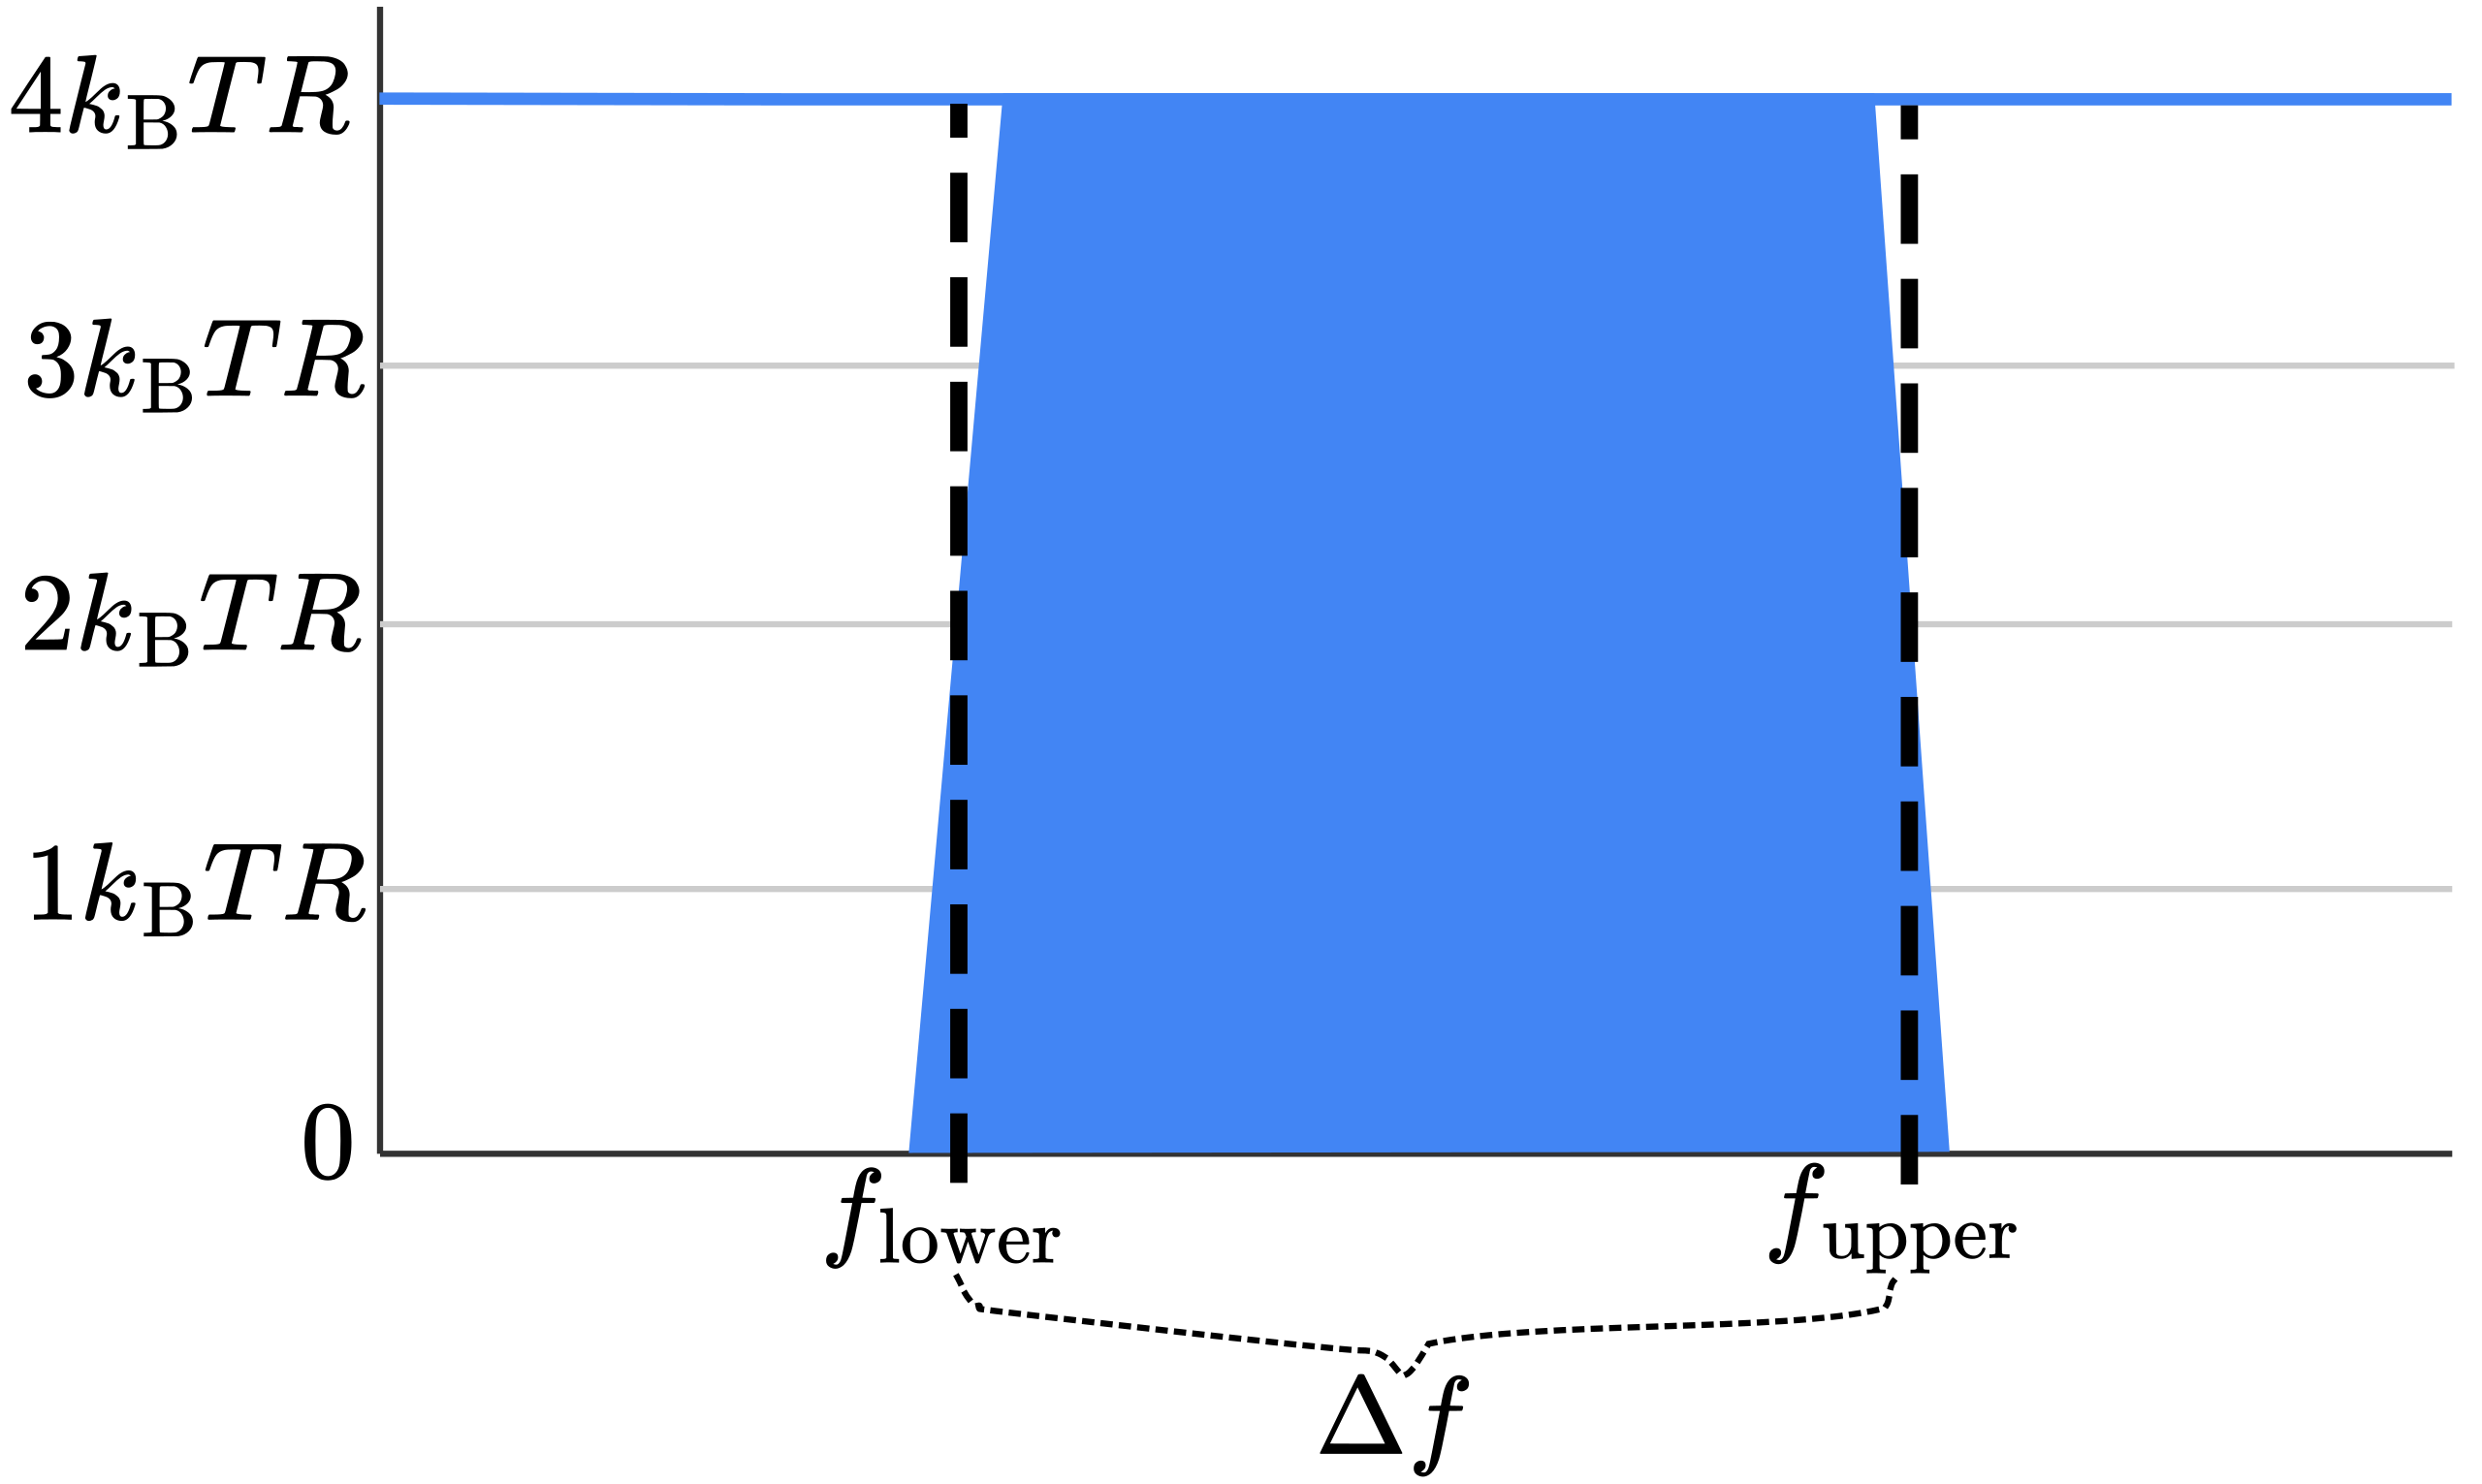
\includegraphics[width=0.4\linewidth]{images/Effect-of-bandwidth-on-selecting-noise}
			\caption{尽管热噪声具有接近常数的功率谱密度$4 k_\text{B} T R$，但带宽为$\Delta f = f_\text{upper} - f_\text{lower}$的带通滤波器只通过高度为$4 k_\text{B} T R$、宽度为$\Delta f$的阴影部分。注意：实际的滤波器没有理想的“砖墙”截止频率，因此该区域的左右边缘并不是完全垂直的。（来自\cite{a}）}
			\label{fig:effect-of-bandwidth-on-selecting-noise}
		\end{figure}
		
		每赫兹带宽的均方电压为$4 k_\text{B} T R$，并且可以称为\textbf{功率谱密度}。在室温（约300 K）下，其平方根近似为$0.13 \sqrt{R}$，单位为$\mathrm{nV}/\sqrt{\mathrm{Hz}}$。例如，一个10 kΩ的电阻在室温下大约具有13 $\mathrm{nV}/\sqrt{\mathrm{Hz}}$。
		
		\begin{figure}[htbp]
			\centering
			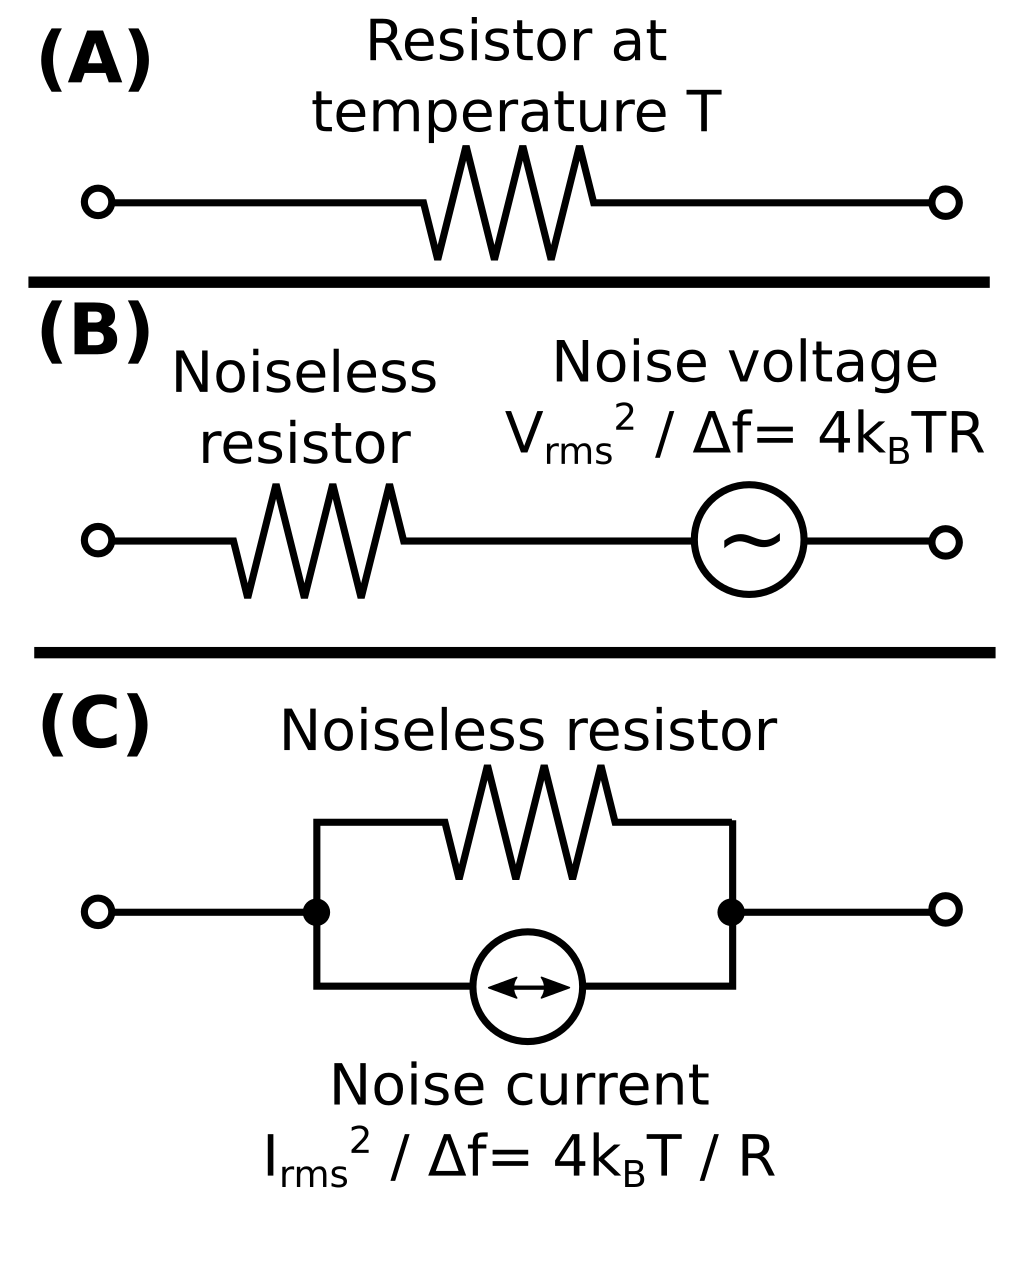
\includegraphics[width=0.3\linewidth]{images/JohnsonNoiseEquivalentCircuits}
			\caption{这些电路是等效的：
				\textbf{(A)} 带有内部热噪声的非零温度电阻；
				\textbf{(B)} 其\textbf{戴维南等效}电路：一个无噪声电阻与噪声电压源串联；
				\textbf{(C)} 其\textbf{诺顿等效}电路：一个无噪声电阻与噪声电流源并联。（来自\cite{a}）}
			\label{fig:johnsonnoiseequivalentcircuits}
		\end{figure}
		
		均方电压的平方根给出了在带宽$\Delta f$上的\textbf{均方根}（RMS）电压：
		\begin{equation*}
			V_\text{rms} = \sqrt{\overline {V_n^2}} = \sqrt{ 4 k_\text{B} T R \, \Delta f } \, .
		\end{equation*}
		
		带有热噪声的电阻可以用其\textbf{戴维南等效电路}表示，包含一个与高斯噪声电压源串联的无噪声电阻，其RMS电压如上所述。
		
		在室温下，3 kΩ的电阻在20 kHz（人类听力范围）带宽上产生的RMS噪声电压几乎为1微伏，$R \, \Delta f$为60 Ω·Hz时，RMS噪声电压几乎为1纳伏。
		
		带有热噪声的电阻还可以\textbf{转换为诺顿等效电路}，其等效电路为一个与高斯噪声电流源并联的无噪声电阻，其均方根电流为：
		\begin{equation*}
			I_\text{rms} = {V_\text{rms} \over R} = \sqrt {{4 k_\text{B} T \Delta f } \over R} \, .
		\end{equation*}
		
		\item 奈奎斯特对理想电阻噪声的推导
		
		\begin{figure}[htbp]
			\centering
			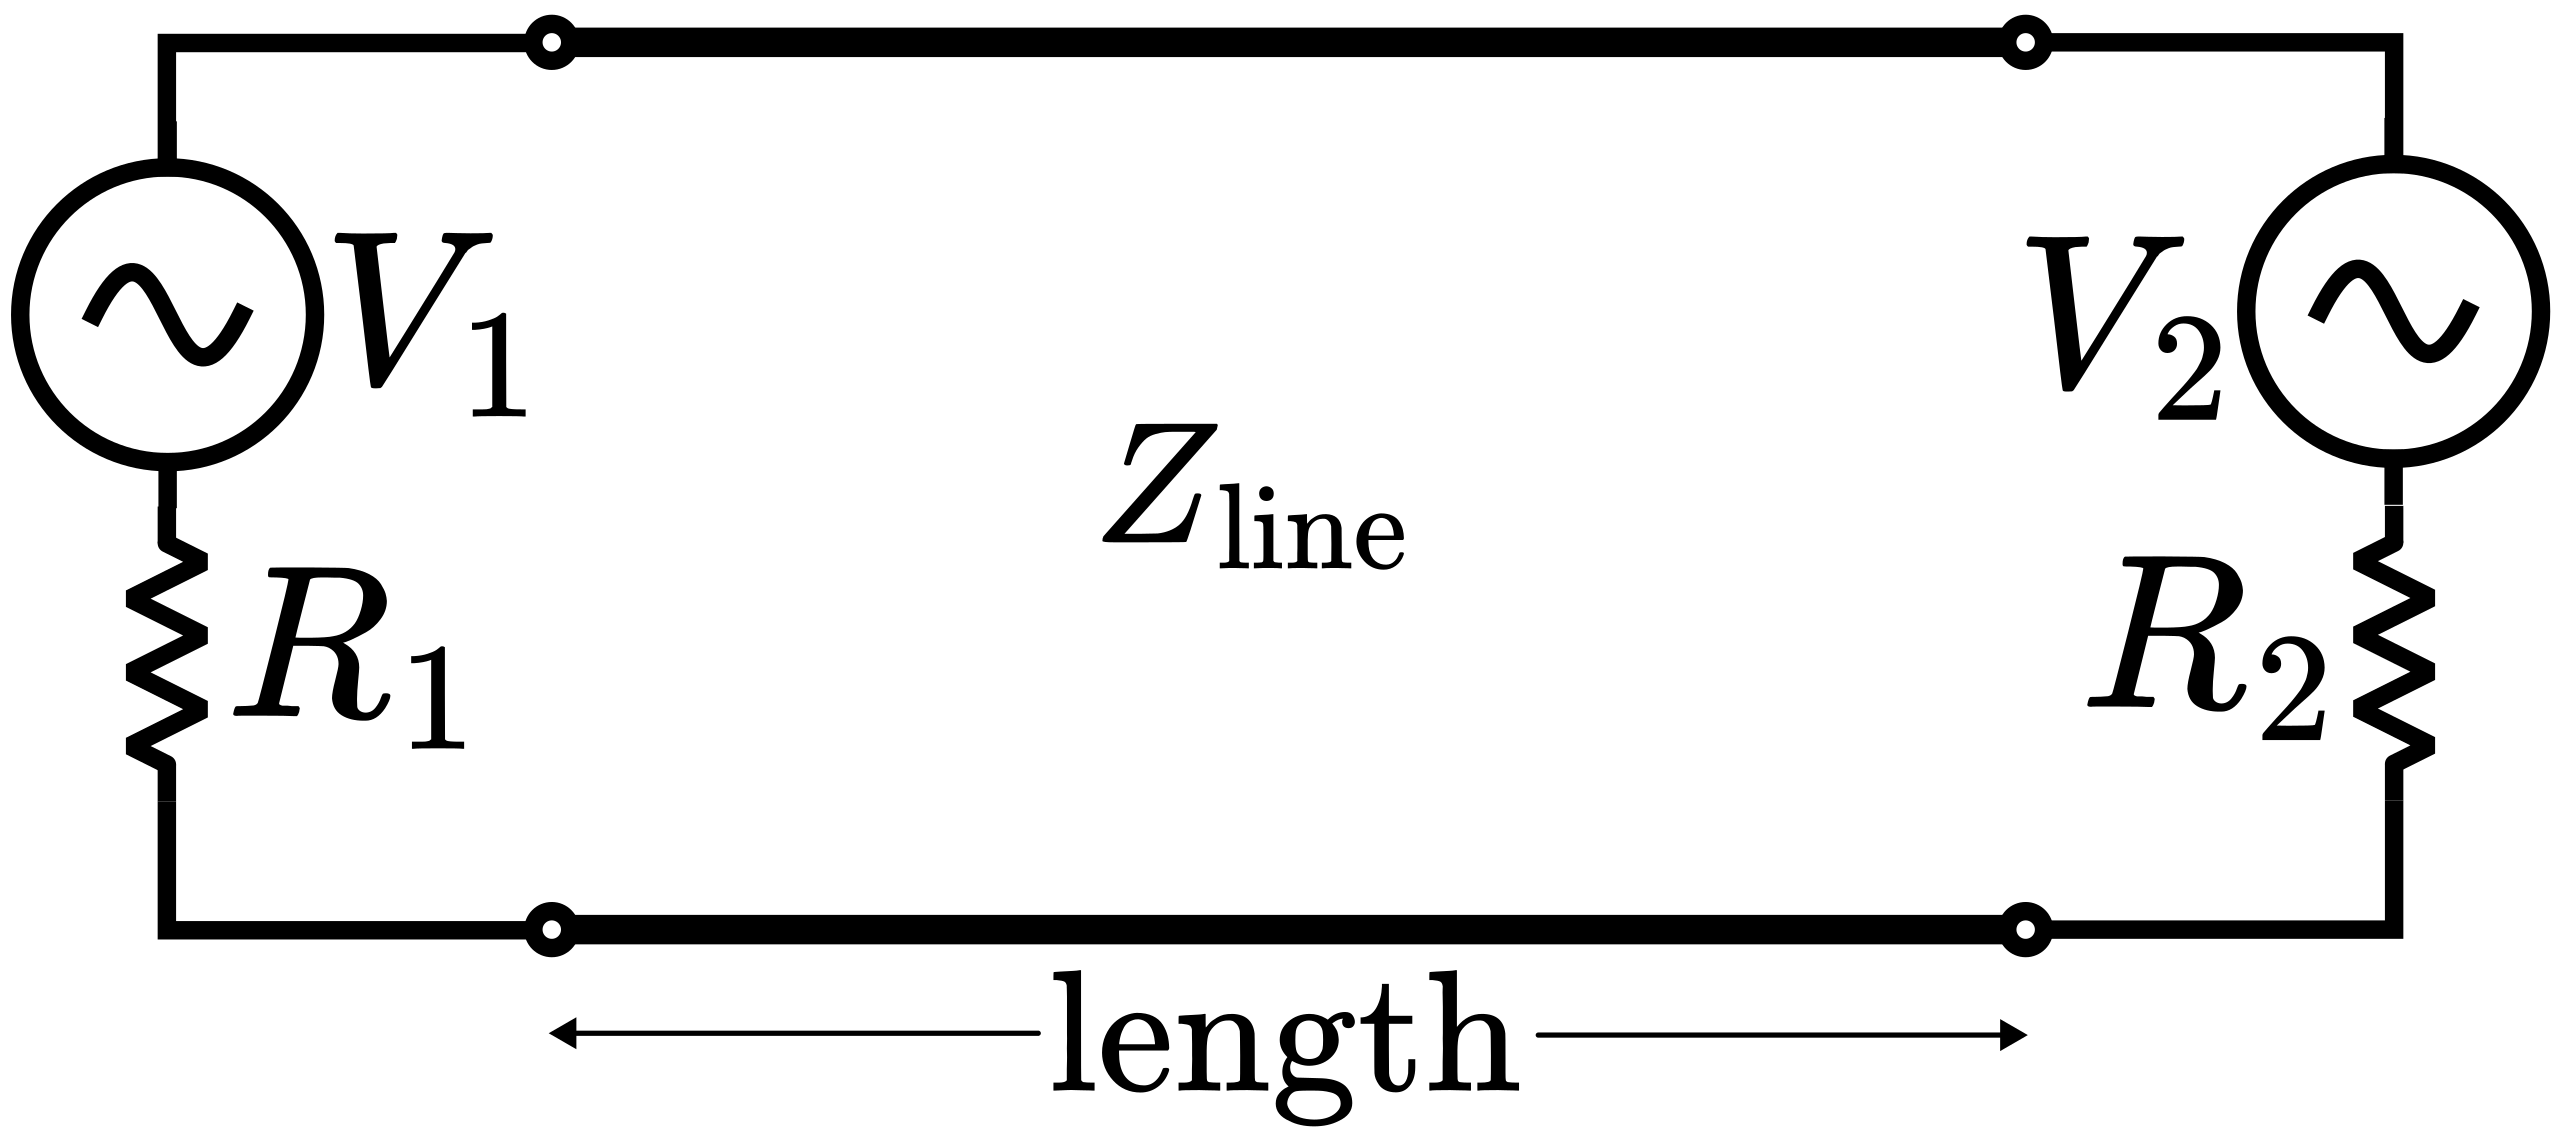
\includegraphics[width=0.4\linewidth]{images/Nyquist-transmission-line-derivation-of-johnson-noise-with-voltage-sources}
			\caption{奈奎斯特于1928年提出的思想实验的示意图。他使用两个有噪声的电阻（每个电阻由无噪声电阻和噪声电压源串联表示）通过一条长度为$l$的无损传输线连接。每个电阻的噪声信号以速度$v$沿传输线传播。由于所有阻抗相同，因此两个信号均被对方的电阻吸收而不是反射。奈奎斯特接着设想将传输线两端短路，从而将在线上运行的能量困住。由于阻抗不匹配，所有在途能量完全反射，此时可以用正弦驻波的叠加来表示这部分能量。在频带$\Delta f$内，有$2l \, \Delta f / v$个振荡模式。每个模式平均提供$k_\text{B} T$的能量，其中一半为电能（$k_\text{B} T / 2$），另一半为磁能，因此该频带内的总能量平均为$k_\text{B} T \cdot 2l \, \Delta f / v$。每个电阻贡献了$k_\text{B} T \cdot l \, \Delta f / v$的能量。由于短路前没有反射，传输线上总的在途能量也等于从两个电阻转移到传输线上的能量之和。除以传播时间间隔$l / v$，每个电阻平均在带宽$\Delta f$上转移的总功率为$k_\text{B} T \, \Delta f$。（来自\cite{a}）}
			\label{fig:nyquist-transmission-line-derivation-of-johnson-noise-with-voltage-sources}
		\end{figure}
		
		奈奎斯特在1928年的论文《导体中电荷的热激发》中，使用了玻尔兹曼和麦克斯韦的能量均分定律中关于势能和谐振子的概念，来解释约翰逊的实验结果。奈奎斯特的\textbf{思想实验}将两个相等电阻（$R_1 = R_2$）之间长无损传输线上的每个驻波模式的能量进行了求和。
		
		$R_1$在带宽$\Delta f$上传输到$R_2$的平均功率为：
		\begin{equation*}
			\overline{P_1} = k_\text{B} T \, \Delta f \, .
		\end{equation*}
		
		$V_1$（仅$R_1$的热噪声电压）通过组合电阻的电流为：
		\begin{equation*}
			I_1 = \frac{V_1}{R_1 + R_2} = \frac{V_1}{2R_1} \, ,
		\end{equation*}
		
		因此，$R_1$传输到$R_2$的功率为该电流的平方乘以$R_2$，简化为：
		\begin{equation*}
			P_1 = I_1^2 R_2 = I_1^2 R_1 = \left( \frac{V_1}{2R_1} \right)^2 R_1 = \frac{V_1^2}{4R_1} \, .
		\end{equation*}
		
		将$P_1$等于之前的平均功率表达式$\overline{P_1}$，可以求出在该带宽上的$V_1^2$的平均值：
		\begin{equation*}
			\overline{V_1^2} = 4 k_\text{B} T R_1 \, \Delta f \, .
		\end{equation*}
		
		\item 涨落耗散定理与电阻器中的热噪声
		
		涨落-耗散定理可以通过多种方式来表述，其中一种特别有用的形式如下：设$x(t)$是一个具有哈密顿量$H_0(x)$的动力系统的\textbf{可观测量}，该系统受到热涨落的影响。可观测量$x(t)$将在其平均值$\langle x\rangle_0$附近波动，这些波动可以通过\textbf{功率谱}$S_x(\omega) = \langle \hat{x}(\omega)\hat{x}^*(\omega) \rangle$来描述。假设我们可以施加一个时间变化的、空间上恒定的场$f(t)$，该场使哈密顿量变为$H(x) = H_0(x) - f(t)x$。可观测量$x(t)$对时间依赖场$f(t)$的响应，可以通过系统的\textbf{磁化率}或\textbf{线性响应函数}$\chi(t)$的一级近似来描述：
		\begin{equation*}
			\langle x(t) \rangle = \langle x \rangle_0 + \int_{-\infty}^{t} f(\tau) \chi(t-\tau) \, d\tau,
		\end{equation*}
		其中，摄动在$\tau = -\infty$时被逐渐（非常缓慢地）引入。
		
		涨落-耗散定理将$x$的双边功率谱（即正频率和负频率）与磁化率$\chi(t)$的傅里叶变换$\hat{\chi}(\omega)$的虚部联系起来：
		\begin{equation*}
			S_x(\omega) = -\frac{2 k_\mathrm{B} T}{\omega} \operatorname{Im}\hat{\chi}(\omega).
		\end{equation*}
		该等式成立的前提是傅里叶变换的约定为$f(\omega) = \int_{-\infty}^{\infty} f(t) e^{-i\omega t} \, dt$。左侧描述了$x$的\textbf{涨落}，右侧则与系统在受到振荡场$f(t) = F \sin(\omega t + \phi)$激励时\textbf{耗散}的能量密切相关。涨落的频谱揭示了线性响应，因为过去的涨落通过线性响应引起未来的涨落。
		
		约翰逊-奈奎斯特噪声，均方电压取决于电阻$R$、$k_{\rm B}T$以及测量电压的带宽$\Delta\nu$：
		\begin{equation*}
			\langle V^2 \rangle \approx 4Rk_{\rm B}T\,\Delta\nu \, .
		\end{equation*}
		
		这一观察可以通过\textbf{涨落-耗散定理}来理解。以一个由电阻$R$和小电容$C$组成的简单电路为例。根据\textbf{基尔霍夫电路定律}，电压满足以下关系：
		\begin{equation*}
			V = -R\frac{dQ}{dt} + \frac{Q}{C} \, .
		\end{equation*}
		
		因此，该电路的\textbf{响应函数}为
		\begin{equation*}
			\chi(\omega) \equiv \frac{Q(\omega)}{V(\omega)} = \frac{1}{\frac{1}{C} - i\omega R} \, .
		\end{equation*}
		
		在低频极限$\omega \ll (RC)^{-1}$下，响应函数的虚部近似为
		\begin{equation*}
			\text{Im}\left[\chi(\omega)\right] \approx \omega RC^2 \, .
		\end{equation*}
		
		通过涨落-耗散定理，可以将其与电压的\textbf{功率谱密度}函数$S_V(\omega)$联系起来
		\begin{equation*}
			S_V(\omega) = \frac{S_Q(\omega)}{C^2} \approx \frac{2k_{\rm B}T}{C^2\omega} \text{Im}\left[\chi(\omega)\right] = 2Rk_{\rm B}T \, .
		\end{equation*}
		
		在带宽$\Delta f = \Delta\omega / (2\pi)$内观察到的约翰逊-奈奎斯特电压噪声$\langle V^2 \rangle$，中心频率为$\omega = \pm \omega_0$。因此
		\begin{equation*}
			\langle V^2 \rangle \approx S_V(\omega) \times 2\Delta f \approx 4Rk_{\rm B}T\Delta f \, .
		\end{equation*}
		
	\end{enumerate}
	
	\item 噪声的测量
	
	实验利用锁相放大器测量噪声。时域上做等时间间隔采样，多次测量计算信号的\textbf{方均根值}。这句话的意思是：设备在等间隔的时间点上读取一个信号 $v(t_i) = s(t_i) + n(t_i)$，$s(t_i)$ 为 $t_i$ 时刻频率为 $f$ 的信号，$n(t_i)$ 为 $t_i$ 时刻的噪声，经与信号同频率 $f$ 的参考信号相敏检波后，输出 X 分量$X_f(t_i) = s_x(t_i) + n_f(t_i)$，是包含“同频”噪声的信号。定义噪声强度 X 分量测量值（这个式子显然是信号的方均根的表达式，同时它表达了噪声电压有效值）：
	\[
	v_{Nx}(f) = \sqrt{\frac{\sum_{i=1}^{M} \left(X_f(t_i) - \bar{X_f}\right)^2}{M}}
	\]
	其中，$\bar{X}_j = \frac{1}{M} \sum_{j=1}^{M} X_j$为输入信号的平均值，$M$ 为用于计算输入噪声值的样本数。
	
	实际测量有各种各样的噪声，考虑按以下方式合成：
	\[
	v_{Nx}(f) = \sqrt{\frac{\sum_{i=1}^{M} \left( n_{f_x}(t_i) \right)^2}{M}} = \sqrt{\frac{\sum_{i=1}^{M} \left( \sum_{k=1}^{m} n_{f_xk}(t_i) \right)^2}{M}} 
	\]
	
	分离不同种类的噪声是困难的，除非在输入端做物理隔离。所以我们考虑的是非相干的噪声，按以下方式做合成：
	\[
	v_{Nx}(f) = \sqrt{\frac{\sum_{k=1}^{m} \sum_{i=1}^{M} \left( n_{f_xk}(t_i) \right)^2}{M}}
	\]
	上式给出了不同类型非相干噪声的叠加原理。
	
	对随机噪声，X 与 Y 独立等价，即输入噪声功率为 X 或 Y 测量功率的 2 倍：
	\[
	v_N^2 = \frac{1}{M} \sum_{j=1}^{M} \left( n_{xT}^2(j) + n_{yT}^2(j) \right) = \frac{2}{M} \sum_{j=1}^{M} n_{xT}^2(j)
	\]
	
	\item 仪器本底扣除及输入带宽修正
	
	测量电阻 $R$ 的噪声 ($n_R$) 是待测热噪声 ($n_T$) 与本底噪声的叠加。根据随机噪声叠加原理式得：
	\[
	n_{Rx}^2(\omega) = n_{Tx}^2(\omega) + n_{Bx}^2(\omega)
	\]
	
	可扣除仪器的本底噪声，\textbf{前提是测量本底噪声时与测量噪声时的条件，以及所选的锁相放大器参数相同}。
	
	事实上，在后续进一步的资料查找阅读过程中，从\cite{g}中了解到如下信息，这进一步对电阻阻值和测温点的参数值的选取提供了参考：
	
	锁相放大器的本底噪声谱密度在 $5 \, \text{nV}/\sqrt{\text{Hz}}$ 左右， 相当于 $6 \, \text{k}\Omega$ 的电阻在液氮温度 (77 K) 下，或 $1.5 \, \text{k}\Omega$ 的电阻在室温 (300 K) 下的热噪声谱密度。可见，要降低热噪声测量的系统误差，一方面要求保证样本量足够大，另一方面电阻值选 $5 \sim 100 \, \text{k}\Omega$ 比较合适。
	
	进一步再考虑输入带宽修正：
	\[
	n_{Tx}^2 = n_{Rx}^2 \left[ 1 + (\omega R_{\text{in}} C_{\text{in}})^2 \right] - n_{Bx}^2
	\]
	其中，$R_{\text{in}}$ 和 $C_{\text{in}}$ 分别为锁相放大器的输入端的等效电阻和等效电容。
	
	带宽修正项 \(1 + (\omega R_{\text{in}}C_{\text{in}})^2\) 反映了输入阻抗和电容对信号频率响应的影响，这个修正项可以通过输入电路的频率响应特性推导出来，特别是输入阻抗 \( R_{\text{in}} \) 和电容 \( C_{\text{in}} \) 所形成的低通滤波效应。锁相放大器的输入端通常有输入电阻和输入电容，这两者并联形成了一个简单的RC电路，对输入信号产生低通滤波作用。假设输入信号电压为 \( V_{\text{in}} \)，在通过该RC电路时会产生频率依赖的输出电压 \( V_{\text{out}} \)。这一过程可以用传递函数来描述为：
	\[
	H(\omega) = \frac{V_{\text{out}}}{V_{\text{in}}} = \frac{1}{1 + j\omega R_{\text{in}} C_{\text{in}}}
	\]
	其中 \( \omega = 2\pi f \) 为角频率，\( j \) 为虚数单位。
	
	为了得到输入信号经过该RC电路后的衰减效果，我们需要计算传递函数的幅值平方：
	\[
	|H(\omega)|^2 = \left| \frac{1}{1 + j\omega R_{\text{in}} C_{\text{in}}} \right|^2 = \frac{1}{1 + (\omega R_{\text{in}} C_{\text{in}})^2}
	\]
	这个结果表示信号经过RC电路后，随频率增高而衰减。
	
	测量电阻热噪声时，电阻产生的噪声信号通过该RC电路，因此噪声的频谱功率密度也会随着频率而衰减。由于热噪声是白噪声，在不同频率下均匀分布，我们需要对测量到的噪声功率进行修正。假设 \( n_{\text{Rx}}^2 \) 是未经修正的噪声功率，那么经过RC电路后的噪声功率会变为：
	\[
	n_{\text{Tx}}^2 = n_{\text{Rx}}^2 \cdot |H(\omega)|^2 = n_{\text{Rx}}^2 \cdot \frac{1}{1 + (\omega R_{\text{in}} C_{\text{in}})^2}
	\]
	
	由于实验的目标是测量未经滤波器影响的噪声信号，因此我们需要将传递函数中的频率衰减效应修正回来。通过乘以传递函数的倒数，可以得到修正后的噪声功率：
	\[
	n_{\text{Tx}}^2 = n_{\text{Rx}}^2 \cdot \left[ 1 + (\omega R_{\text{in}} C_{\text{in}})^2 \right]
	\]
	这样我们就补偿了输入电路对噪声信号的衰减效应，得到接近理想条件下的噪声功率。
	
	此外，锁相放大器自身产生的本底噪声也需要从测量结果中扣除，假设本底噪声的功率为 \( n_{\text{Bx}}^2 \)，最终修正后的噪声功率为：
	\[
	n_{\text{Tx}}^2 = n_{\text{Rx}}^2 \left[ 1 + (\omega R_{\text{in}} C_{\text{in}})^2 \right] - n_{\text{Bx}}^2
	\]
	
	为什么本底噪声不必做输入带宽修正？本底噪声是锁相放大器内部的固有噪声，不经过外部输入电路，因此不会受到输入带宽的影响，也无需进行带宽修正。而外部噪声，如电阻的热噪声，会受到输入阻抗和滤波器的影响，因此需要进行带宽修正。
	
	此外，注意讲义上提到的非随机的环境噪声$n_{ex}$。
	
	实验讲义上提供了具体的数值：影响输入带宽的 $R_{\text{in}}$ 约为 $2/3R$，$C_{\text{in}}$ 约为电缆电容（室温下约为 96pF/m）、锁相放大器输入电容（25pF），与包括连接器和样品盒在内的电容并联后的值的 1/2（约 \textbf{68pF}）。
	
	\item $k_B$的计算
	
	首先考虑\textbf{等效噪声带宽}。实际滤波器带宽做不到理想的矩形，我们用谱线所包围的功率面积等于矩形面积来定义等效噪声带宽，等效噪声带宽 $\text{ENBW} = \Delta f_{\text{LPF}}/2$ 。将随机变化的噪声看作幅值随时间的阶跃输入信号，则窄带滤波器使输出信号延迟。定义输出信号达到阶跃的 99\% 视为反映输入噪声幅值，其延迟或等待时间也列于\cref{tab:ENBW}。$X$ 稳定需要的等待时间为 $t_X$。
	
	\begin{table}[h!]
		\centering
		\caption{单分量等效噪声带宽（ENBW）与陡降和时间常数$\tau$的对应关系}
		\label{tab:ENBW}
		\begin{tabular}{cccc}
			\hline
			\textbf{阶数(n)} & \textbf{Slope (dB/oct)} & \textbf{ENBW (1/$\tau$)} & \textbf{X 测量等待时间$t_X$}\\
			\hline
			1 & 6 & 1/4 & 4.6 \\
			2 & 12 & 1/8 & 6.6 \\
			3 & 18 & 3/32 & 8.4 \\
			4 & 24 & 5/64 & 10 \\
			\hline
		\end{tabular}
	\end{table}
	
	\textbf{注意ENBW需要通过计算得来，根据不同的陡降得到不同的系数（来自讲义的表），在乘以时间常数的倒数便得到带宽。}
	
	引入ENBW后，我们可以得到最终\textbf{玻尔兹曼常数的计算式}。考虑到，$v_N$ 测量值与仪器带宽有关，故用与仪器参数无关的噪声谱密度描述噪声特性应：
	\begin{ubox}{}
		$$
		S_T(f)=v_{Nx}/\sqrt{\text{ENBW}} = \sqrt{4k_BTR} \Rightarrow k_B = \dfrac{v_{Nx}^2}{4\times\text{ENBW}\times TR}
		$$
	\end{ubox}
	
	作为参考，1.0k$\Omega$金属电阻在室温 (300K) 下噪声谱密度为：
	\[
	\sqrt{4 \times 1.38 \times 10^{-23} \text{J/K} \times 300\text{K} \times 1000\Omega} = 4.07\text{nV}/\sqrt{\text{Hz}}
	\]
	
	此外，基于$k_B = \dfrac{v_{Nx}^2}{4\times\text{ENBW}\times TR}$，我们可以考虑一种变温测量下的\textbf{线性拟合方案}，即用变化的温度与阻值（阻值也会随温度变化）乘积作为梯度测量下的功率谱变化的斜率以表征玻尔兹曼常数：
	$$
	\dfrac{v_{Nx}^2}{\text{ENBW}}=4k_B\times TR
	$$
	
	实际测量 $S_T(f)$ 时，锁相放大器采样次数不可能无限大，热噪声测量值的比值标准差与样本量的关系约为 $2/\sqrt{M}$。
	
	此外，OE1022 锁相放大器用式计算噪声电压谱密度（$N$ 值）的样本量为 1024 个。受限于低通滤波器，所测得的邻近两个 $N$ 值不一定是独立无关的，从而电压数据也未必服从正态分布。因此，\textbf{建议实验时直接记录 X 或 Y，再计算噪声强度和噪声谱密度更为清晰可靠。}
	
\end{enumerate}


%---------------------------------------------------------------------
% 实验前思考题
\subsection{Thinking Before Experiment}

% 思考题1
\begin{question}
	如何与同班组的同学分配频率点？
\end{question}
在分配频率点时，合理的分配能够确保实验的顺利进行，同时避免重复测量和资源浪费。首先，我们需要确定测量的频率范围和步进，通常根据实验要求和设备限制确定。如果讲义中没有明确规定频率范围，通常可以根据设备性能自行选择适合的范围，例如1 Hz到100 kHz。之后根据班组人数，合理分配频率点。假设一个实验组有4名同学，可以采用线性划分或对数划分的方式分配频率点。

在线性划分的方案中，频率点均匀分布在每个人负责的范围内。例如，在1 Hz到100 kHz的频率范围内测量20个频率点，每个同学负责其中的5个频率点。具体分配可以是：同学A测量1 Hz、10 Hz、100 Hz、1 kHz、10 kHz，同学B测量2 Hz、20 Hz、200 Hz、2 kHz、20 kHz，依此类推。这种分配方式简单易行，并确保每位同学都有从低频到高频的覆盖。

另一种方式是对数划分，适合频率跨度较大的实验。对于频率范围从1 Hz到100 kHz的情况，可以选择在对数坐标上均匀分配频率点。例如，16个频率点可以按对数划分，每个同学负责如1 Hz、10 Hz、100 Hz、1 kHz等倍数变化的频率点，这样的划分方式能够更好地覆盖高频段的变化。同时，低频点也会保持合理的间隔。

无论采用何种方案，都建议不同同学在某些频率点上进行交叉验证，以确保数据的一致性和准确性。例如，同学A和同学B可以在10 Hz和1 kHz进行重复测量，同学C和D则在50 Hz和5 kHz交叉测量。这样可以及时发现可能存在的误差，提高实验数据的可靠性。

% 思考题2
\begin{question}
	在测量所选参量前或后，是否需要对锁相放大器进行校正？如何校正？
\end{question}
在进行电阻热噪声和玻尔兹曼常量测量的实验中，校正锁相放大器是确保测量准确性的关键步骤。由于实验涉及微弱信号和噪声的测量，锁相放大器的参数校正尤为重要。这些校正步骤可以帮助消除设备本身的误差，提高实验的精确性。

首先，锁相放大器的零点校正是一个必要的步骤。当没有信号输入时，锁相放大器可能会显示一定的输出电压，这通常是由于零点漂移引起的。因此，校正零点的过程通常包括断开输入信号，使输入端短接或断开，并通过调节放大器的偏移设置，将输出调整为零。这一步能够确保在没有输入信号时，放大器的输出保持为零，避免由于零点漂移而带来的测量误差。

其次，本底噪声的校正在实验中也是至关重要的。锁相放大器自身存在一定的本底噪声，这包括热噪声、温漂噪声以及模数转换噪声等。当进行噪声测量时，测得的噪声信号不仅包含来自外部电阻的热噪声，还包含设备本身的噪声。因此，在测量外部信号前，需要先测量设备的本底噪声，并记录其平方值 \( n_{\text{Bx}}^2 \)。在后续实验中测量总噪声 \( n_{\text{Rx}}^2 \) 后，使用公式
\[
n_{\text{Tx}}^2 = n_{\text{Rx}}^2 \left[ 1 + (\omega R_{\text{in}}C_{\text{in}})^2 \right] - n_{\text{Bx}}^2
\]
扣除设备的本底噪声，从而得到真实的噪声信号。通过这种方式，能够有效地消除本底噪声对实验结果的影响，确保测量的准确性。

增益校正也是实验中必不可少的步骤。增益的准确性直接影响到测量微弱信号时的幅值精度。为了校正增益，可以输入一个已知幅值的正弦信号，观察放大器的输出信号是否与输入信号一致。如果输出信号的幅值偏差较大，可以通过调整锁相放大器的灵敏度（Sensitivity）和增益（Gain）设置，使得输出信号与输入信号的已知幅值匹配。通过这种方式，可以确保放大器的增益是准确的，尤其是在使用不同电阻值或测量微弱信号时，增益的准确性至关重要。

在每个实验阶段，尤其是测量不同电阻值或温度点时，定期对设备进行校正是必要的。通过校正，可以确保锁相放大器的工作状态稳定，避免由于设备参数的变化而影响实验结果。

% 思考题3
\begin{question}
	如何辨别在某频率下测量到的噪声是电阻本身的热噪声还是带有环境噪声？
\end{question}
在辨别电阻热噪声和环境噪声时，可以利用噪声的频率特性进行区分。根据讲义的内容，电阻的热噪声是典型的白噪声，其功率谱密度与频率无关，呈现出平坦的分布。而环境噪声，如市电干扰，则通常具有特定的频率成分，常见的频率峰值出现在 50 Hz 及其倍频（如 100 Hz、150 Hz）。通过对不同频率点的测量，可以观察到环境噪声在这些特定频率上的峰值。如果在这些频率处出现了显著的噪声增强，就可以判断噪声中含有环境噪声成分，而热噪声应该在整个频谱中均匀分布。

根据讲义中提到的本底噪声校正方法，锁相放大器本身带有一定的本底噪声，包括设备的热噪声和温漂噪声等。因此，测量的总噪声是电阻热噪声与本底噪声的叠加。为了更准确地获得电阻的热噪声，需要在断开信号输入的情况下测量本底噪声，记录并扣除该值。这可以有效减少设备本身对实验结果的干扰，从而得到更加接近真实热噪声的测量结果。

通过调整锁相放大器的带宽，也可以帮助排除环境噪声的干扰。热噪声的强度随带宽线性变化，因此如果噪声信号随带宽增加而线性增加，可以判断噪声主要是电阻的热噪声。如果噪声随带宽变化不呈线性关系，尤其是在某些频段内波动较大，则很可能是环境噪声的影响。此外，使用法拉第笼等屏蔽措施可以有效隔离外界电磁干扰，这在实验中也有助于区分热噪声和环境噪声。通过屏蔽外界的电磁干扰，可以显著减少环境噪声的影响，使得测量的信号更加准确反映电阻的热噪声特性。

最后，实验中还可以通过合理安排实验时间来减少环境噪声的干扰。讲义中提到，环境噪声在工作日白天较为明显，因此可以选择在夜间或设备较少的环境中进行测量，这样可以减少环境噪声的干扰，确保测得的噪声主要来自电阻的热噪声。

事实上，\cite{c}已经提到，环境噪声会对测量结果造成不小的影响（这一点后面也会讨论）。
